\chapter{Usabilidade}

	Neste capítulo abordaremos os conceitos e as áreas que estão por trás do termo usabilidade e as relações entre cada uma delas.Entender a importância e os benefícios que a usabilidade trás para os sistemas de software. Apresentar os modelos de ciclo de vida utilizados na interação humano computador e mostrar como podemos inserir a usabilidade no ciclo de desenvolvimento de software empírico.

\section {Usabilidade}

	A usabilidade é um termo antigo que começou a ser utilizado pela Ciência Cognitiva e depois pela Psicologia e Ergonomia em substituição ao termo “amigável” ~\cite{dias2006}.

	A usabilidade é um atributo de qualidade relacionado à facilidade de uso de algo. Refere-se a rapidez com que os usuários podem aprender a usar alguma coisa, a eficiência deles ao usá-la, o quanto lembram daquilo, seu grau de propensão a erros e o quanto gostam de utilizá-la ~\cite{nielsen2007}. .

	Uma outra definição de usabilidade é a capacidade do produto de software ser compreendido, aprendido, operado e atraente ao usuário, quando usado sob condições específicas ~\cite{iso9126-1}

	A Qualidade em uso engloba o contexto do ambiente de trabalho para caracterizar a satisfação de uso, focando não apenas no usuário, mas em seu comportamento ao interagir com um sistema computacional.

	O conceito de qualidade em uso mais difundido é o de usabilidade que engloba a facilidade e a eficiência de aprendizado de uso, bem como a satifação do usuário. 	
%Falar da qualidade em uso
	
	Ainda usabilidade é definida como o fator que assegura que um produto ou serviço é fácil de usar, eficiente e agradável a partir do ponto de vista do usuário ~\cite{preece2007}.

	Segundo Jakob Nielsen, usabilidade é um conjunto de propriedades de uma interface que reúne os seguintes componentes: fácil aprendizado, eficiência, capacidade de memorização, baixo índice de erros e satifação e prazer ao uso.

	Segundo a ~\citeonline{iso9241-11}, usabilidade é a capacidade de um produto ser usado por usuários específicos para alcançar objetivos específicos com eficácia, eficiência e satisfação em um contexto de uso específico.A iso define alguns termos que são amplamente utilizados quando se fala em usabilidade.

\begin{itemize}
\item \textbf{Eficácia} é a capacidade que os sistemas conferem a diferentes tipos de usuários para alcançar seus objetivos em número e com a qualidade necessária. 
\item \textbf{Eficiência} é a quantidade de recursos que os sistemas solicitam aos usuários para a observação de seu objetivos com o sistema.
\item \textbf{Satisfação} é a emoção que os sistemas proporciona, aos usuários em face dos resultados obtidos e dos recursos necessários para alcançar tais objetivos. 
\item \textbf{Tarefa:} Objetivo a ser atingido ou um resultado a obter.
\item \textbf{Usuários:} Pessoas que utilizam alguma instãncia do sistema,
\item \textbf{Contexto:} Conjunto de elementos, onde se destacam: o ambiente físico, a tecnologia utilizada e a a motivação.
\end{itemize}


\begin{figure}[h]
    \centering
    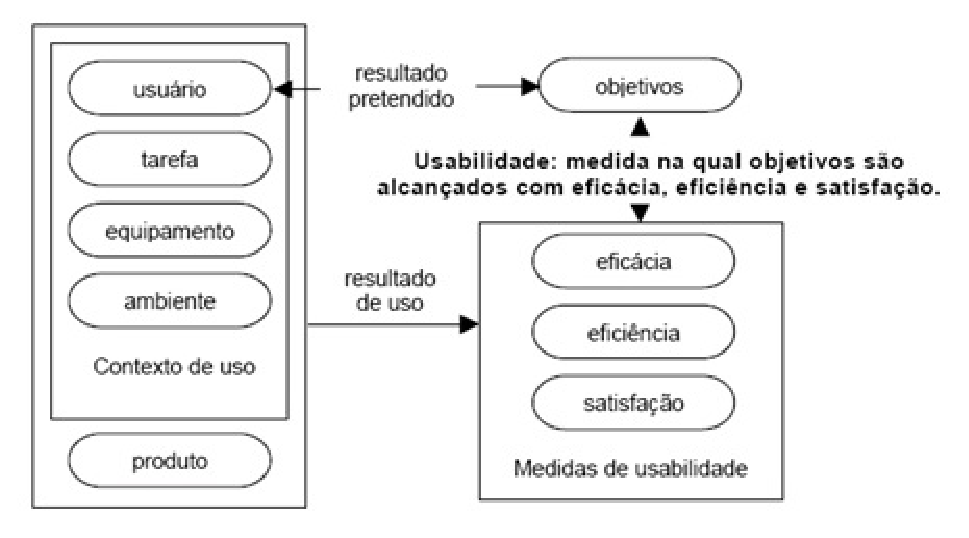
\includegraphics[keepaspectratio=true,scale=0.60]
      {figuras/estruturausabilidade9241.eps}
    \caption{Estrutura de Usabilidade Norma ISO 9241 ~\cite{cybis2010ergonomia}}
    \label{tdd_ciclo}
\end{figure}

\subsection{Metas de Usabilidade}

	As metas de usabilidade servem para guiar o desenvolvimento de produtos fáceis de usar, eficientes e agradáveis ~\cite{preece2007}. São elas:

\begin{enumerate}
\item Utilidade
\item Eficácia
\item Eficiência
\item Segurança
\item Facilidade de aprendizado
\item Facilidade de lembrar como se usa
\end{enumerate}


\section{As áreas da Usabilidade}

	Para entender o que é usabilidade e como ela está inserida no ciclo de vida do desenvolvimento de software precisamos compreender as relações que o termo tem com as diversas áreas que a envolve. 

\subsection{Interação Humano Computador}

	O Termo Human Computer Interaction  (HCI) começou a ser adotado na década de 1980 para descrever uma nova área de estudo na qual se preocupavam em saber como o uso dos computadores poderia enriquecer a vida pessoal e profissional dos seus usuários ~\cite{moraes2002}.
 
	A interação humano computador tem o principal objetivo de melhorar a eficácia e proporcionar satisfação do usuário.O objetivo do HCI são desenvolver e aprimorar sistemas computacionais nos quais os usuários possam executar tarefas com segurança, eficiência e satisfação ~\cite{preece2007}.
	
\subsection{Arquitetura da Informação}

A informação é algo que está presente no nosso dia-a-dia. Para (Wurman, 1991) a informação deve ser aquilo que leva à compreensão. A quantidade de conteúdo que é produzido na internet extrapola a capacidade humana de retenção da informação ~\cite{rosa2012}. Esse excesso de informação contribui para o aumento dos problemas de usabilidade e da necessidade de pesquisa na área de interação humano-computador (Agner, 2004).

Segundo Garrett, a arquitetura da informação são a arte e a ciência de estruturar e organizar os ambientes informacionais para ajudar as pessoas a encontrarem e administrarem informações ~\cite{garret2003}.

O arquiteto de informação deve ser um profissional multidisciplinar com conhecimentos em design gráfico, ciência da informação, biblioteconomia, jornalismo, engenharia de usabilidade, marketing e ciência da computação. Ele deve balancear as necessidades do usuário com os objetivos do negócio ~\cite{rosenfeld1998}.

\subsection{Ergonomia}

A ergonomia está na origem da usabilidade, pois visa proporcionar eficácia e eficiência, além de bem-estar e saúde do usuário através da adaptação do trabalho ao homem. O seu objetivo é garantir que sistemas e dispositivos estejam adaptados às maneiras de pensar, agir e trabalhar do usuário. ~\cite{cybis2010}

	Os fatores físicos, cognitivos, sociais, organizacionais e ambientas são levados em conta na ergonomia por promove uma abordagem holística."A ergonomia está interessada em utilizar as ciências para melhorar as condições de trabalho humano."    

\subsection{Design Centrado no usuário}

	Design centrado no usuário é um campo de estudo que reúne metodologias de design nas quais o público álvo de um produto ou serviço influencia as diretrizes e requisitos do sistema. % fonte slide
	
	Para Don Norman, cunhador do termo, o design centrado no usuário é uma filosofia baseada nas necessidades e interesses dos usuário, com ênfase em fazer produtos úsaveis e inteligíveis.

	Segundo Dan Saffer as pessoas que utilizarão um produto ou serviço sabem de suas necessidades, metas e preferências, e é papel do design descobrir isto e projetar para eles e essa é a filosofia por trás do design centrado no usuário.
	
\subsection{Design de Interaçao}

	Uma grande parte dos produtos que necessitam da interação do usuário são feitos olhando apenas na perspectiva da engenharia e se esquecem de seus reais usuários.O design de interação surge para redirecionar a preocupação que se tinha apenas em produzir algo que funcionasse para produzir algo que sejá fácil de utilizar, agrádavel e eficaz na perspectiva do usuário, trazendo a usabilidade para dentro do processo de design ~\cite{preece2007}.

	Segundo Moggridge, 2006 o termo surgiu com Bill Verplank que resume design de interação a partir da resposta de três perguntas sobre como você age, como você sente e como você compreende. Verplank explica que o design de interação está centrado no usuário, na pessoa e na forma como ela interage com o mundo.
	
	Uma outra definição encontrada consiste em que o design de interação é o design de produtos interativos que fornecem suporte à atividades cotidianas das pessoas, seja no lar ou no trabalho.É criar experiências que melhorem, estendem a maneira como as pessoas trabalham, se comunicam e interagem ~\cite{preece2007}.

	O design de interação é um campo multidisciplinar que centraliza e integra as diversas áreas de conhecimento relacionada a interação entre artefato e usuários.

% colocar figura.

%	Winograd, design de interação é o projeto de espaços para a comunicação e interação humana	
	
%	Existe alguma abordagens que
%	O design de interação pode ser visto por três pontos de vistas segundo Saffer, 2010


% verificar a fonte com Erico Fileno, 2008



\subsection{Engenharia de Usabilidade}

A engenharia de usabilidade surgiu no final dos anos 80 com o esforço sistemático das empresas e organizações para desenvolver programas de software interativo com usabilidade. Sua origem parte de iniciativas de cientistas como Card, Moran e Newell (Modelo do processador Humano de 1983) e Norman (Teoria da Ação de 1989). O objetivo era produzir conhecimentos que favorecesse a concepção de interfaces humano-computador mais adaptadas ~\cite{cybis2010}.

Podemos fazer um paralelo da engenharia de usabilidade com a engenharia de software. A engenharia de software ocupa do desenvolvimento do núcleo funcional de um sistema interativo formado por estruturas de dados, algoritmos e recursos de processamento de dados. Esse núcleo é construído de forma que o sistema funcione bem, de forma correta, rápida e sem erros. Já a engenharia de usabilidade ocupa-se da interface com o usuário que interliga as funções do sistema com os usuários de forma que a interface do sistema seja agradável, intuitivo, eficiente e fácil de operar ~\cite{cybis2010}.



\subsubsection{Ciclo de Engenharia de Usabilidade}

	O ciclo foi definido sendo essencialmente evolutivo, interativo e baseado no envolvimento do usuário. A norma ISO 13407 (Projeto centrado no usuário) sugere quatro principais etapas desse ciclo (analisar e especificar o contexto de operação; especificar as exigências dos usuários e organizações; produzir soluções de projeto; avaliar o projeto contra as exigências) ~\cite{cybis2010}.

%Colocar figura: Projeto centrado no usuário

\subsection{Experiência do Usuário - UX}

	Experiência do usuário é toda a interação que temos com um produto, serviço ou marca. O termo é usado frequentemente para sintetizar toda a experiência com um produto de software. Não engloba  somente nas funcionalidades e sim o quanto o aplicativo é cativante e agradável de ser usado ~\cite{travis2013}.
	
	O termo User Experience (UX) foi cunhado por Donald Norman na década de 80 para......Ele disse atualmente que não gosta do termo pois está sendo utilizado para resumir tudo o que ele estava fugindo, que é pensar em UX como apenas as disciplinas.UX não é uma disciplina é uma cultura.

	Muitas pessoas atribuem ao design para fazer a experiência do usuário, mas UX não é apenas uma etapa e sim deve ser feito por qualquer membro da equipe. Qualquer pessoa envolvida no projeto precisa atuar na experiência do usuário e deve ser feito em todo o 
processo.
	
	Experiência do usuário é resultado de como o produto se comporta quando é usado no cotidiano.Trata de como um produto funciona por fora, onde uma pessa 	


\subsection{Relação de todas essas áreas com a Usabilidade}

	São várias as áreas que envolve-se com o termo usabilidade.A usabilidade está relacionada com os fatores humanos e corresponde como o estudo de como os seres humanos se relacionam com qualquer produto. A interação humano computador está baseada na usabilidade e foca no modo como os seres humanos se relacionam com os produtos ligados à computação.

	Todas essa áreas que envolve a usabilidade de sistemas têm um ponto em comum, o usuário como o foco principal.

	As áreas que trabalham com usabilidade são disciplinas transversais que agregam diversas áreas do conhecimento tais como pscicologia, sociologia, ciência da informação e da computação, fatores humanos, design gráfico e indústrial, ergonomia, comunicação e etc.

% acrescentar mais coisas
%colocar a figura da relação entre usabilidade, ihc dcu e ux
	 
%------------------------------------------------------------------------------%

\section{A importância e os benefícios da Usabilidade}

No modo geral, os projetistas sabem da importância de desenvolver com enfoque no usuário e na usabilidade, mas normalmente os projetos são desenvolvidos sem que tenham sido realizadas pesquisas e aplicados métodos e técnicas de usabilidade.
	
	O tempo e os recursos limitados são as principais razões que impede a implatação dos testes de usabilidade nas equipes de software. Também há o desconhecimento por parte da equipe de desenvolvimento das técnicas a serem empregadas.

Incorporar a usabilidade no seu processo pode reduzir os custos e tempo de desenvolvimento e melhorar o produto final. Ter em mente  em quem é o usuário final em todas as etapas de desenvolvimento e processos de produção, desde análise das necessidades e projeto conceitual até prototipagem e produção.  (reescrever)

	O investimento na área de usabilidade agrega valor ao produto e traz beneficios não somente aos usuários, mas também aos seus produtores. 

Para a Associação de Profissionais de usabilidade (UPA), a usabilidade inclui os seguintes benefícios:

\begin{itemize}
\item Aumentar a produtividade
\item Diminuir custos de treinamento e suporte
\item Aumentar as vendas e as revendas
\item Reduzir os custos de desenvolvimento e manutenção.
\item Aumentar a satisfação do consumidor.
\end{itemize}


%------------------------------------------------------------------------------%. 

\section {Avaliação de Usabilidade}

	
	Os métodos de avaliação são utilizados para avaliar a qualidade das interações entre o usuário e o sistema.São utilizados para verificar, inspecionar e diagnosticar os aspectos ergonômicos das interfaces.

	As avaliações de interface podem ser divididas de diversas maneiras como o tipo de dados, formas e o local da avaliação.

	Quanto a forma pode ser definida como:

	\begin{itemize}
		\item \textbf{Objetiva:} São baseadas em técnicas que utilizam medições quantitativas, em vez de opiniões dos usuários ou especialistas.
		\item \textbf{Subjetiva} São baseadas em opiniões e relatos de usuários e especialisatas.
	\end{itemize}

	Quanto ao tipo de dados pode ser definida como:

	\begin{itemize}
		\item \textbf{Quantitativa} Envolvem medidas e tendem a ser vistas como objtivas e imparciais.
		\item \textbf{Qualitativa} Envolvem descrições e relatos e são vistas como subjetivas.
	\end{itemize}

	Quanto ao local da avaliação:

	\begin{itemize}
		\item \textbf{Laboratório} Ocorre em ambientes controlados.
		\item \textbf{Estudo de Campo ou natural} Estão situados no contexto do mundo real no qual o sistema é utilizado.
	\end{itemize}

	 
	Antes de definir as técnicas de avaliação ~\citeonline{preece2007} identifica quatro tipos de paradigmas de avaliação: (1) avaliações rápidas e sujas; (2) testes de usabilidade; (3) estudos de campos e; (4) avaliações preditivas.

	Em relação as técnicas de avaliação, ~\citeonline{preece2007} as divide em cinco técnicas de avaliação: (1) observação e monitoramento; (2) opinião dos usuários; (3) opiniões dos especialistas; (4) testes com os usuários e; (5) Predição. 

	Já ~\citeonline{cybis2010} divide as técnicas de avaliação da usabilidade de interfaces em três grupos. Técnicas prospectivas; técnicas preditivas/diagnósticas/analíticas/inspecção e as objetivas/definitivas/empíricas.

	De acordo com ~\citeonline{preece1994} cada método de avaliação possui características e pode ser aplicado em diferentes situações.Eles diferem entre si em vários aspectos. É preciso entender as diferentes caracterśiticas de cada método para se definir qual deles é o mais apropriado para avaliar a interface de um software em um determinado contexto. Cada método pode se diferenciar pela etapa do ciclo que pode ser aplicado, a técnica utilizada para coletar dados e os tipos de dados coletados (quantitativa ou qualitativa).

	% colocar tabela com os paradigmas e as técnicas utilizadas ou algo do tipo.

\section{Técnicas e Métodos da Engenharia de Usabilidade}

	Esta seção mostra as técnicas e os métodos que são utilizados pela interação humano computador para desenvolver um sistema com usabilidade.

	De acordo com CERVO e Bervian (2002) as técnicas são procedimentos específicos utilizados por uma ciência determinada.O conjunto com várias técnicas constituem os métodos. Algumas técnicas são utilizadas em várias ciências e os métodos se adapta às diversas ciências a medida que há imposição de uso de técnicas especializadas.

	~\citeonline{cybis2010} divide as técnicas e os métodos da engenharia de usabilidade em três tipos: Concepção, Análise e Avaliação.

\subsection{Métodos e técnicas de concepção}

Os métodos de concepção são utilizados para implementar as especificações e os requisitos para a interface a usabilidade de um sistema.

\subsubsection{Brainstorming}

	O brainstorming é bastante utilizado em ambientes ágeis para obter ideias, entrar em consenso sobre problemas ou novas propostas.

\subsubsection{Storyboard}

É uma representação das interações entre os usuários e o sistema em seu ambiente de trabalho. Corresponde ao detalhamento de um cenário de uso especificado para o sistema consistindo em uma sequência de desenhos representando não só os esboços de telas, mas também os elementos do contexto (usuários, equipamentos, móveis, telefones, colegas).

\subsubsection{Card Sorting}

	É uma técnica usada para descobrir como o usuário classifica determinada informação em sua mente. O usuário recebe uma série de cartões embaralhados descrevendo conteúdos e agrupam os cartões que tenham alguma relação. Podem ser distribuidos cartões com nomes de categorias.
	
	O card sorting pode ser aberto ou fechado podendo ser aplicaso tanto de forma presencial ou remota e aplicados para grupos ou para uma única pessoa.Recomenda-se no mínico 15 testes e que cada teste tenha 2 pessoas.
	
\subsubsection{Diagramas de Afinidade}

	Os diagramas de afinidade são utilizados para organizar uma grande quantidade de itens em grupos lógicos. Diferente do card sorting, nesta técnica os projetistas e usuários trabalham juntos para obter consenso sobre a organização dos itens. Essa técnica pode ser usada para analisar os resultados de estudos de campo e analisar as conclusões de uma avaliação de usabilidade.

\subsubsection{Protótipos}

	Os protótipos de papel é útil para detectar problemas  de usabilidade logo no início do proceso de design. São usados para esclarecer os requisitos específicos para o projeto da interface do sistema.
	São rápidos de construir, permitindo rápidas interações de projeto e necessitam de poucos recursos para serem criados. 
	Existem também os protótipos de baixa, média e alta que simulam o sistema com mais fidelidade do que os protótipos em papel. 

%------------------------------------------------------------%%%

\subsection{Métodos e técnicas de análise}

Estes métodos são utilizados para buscar informações sobre o contexto de uso e sobre a usabilidade de um sistema. Podem ser feitas análises do perfil do usuário, o ambiente de uso, as tarefas, possibilidades e restrições do sistema.

As técnicas mencionadas à baixo visam apoiar os projetistas de interface na busca de informações sobre o contexto de uso e sobre a usabilidade de um sistema existente. Essas técnicas são empregadas de forma que se complementem-se umas as outras.

As entrevistas tradicionais e os questionários combinam resultados qualitativos e quantitativos para permitir melhor compreensão do “perfil do usuários”.
	
%Verificar pg 173, livro cybis

\subsubsection{Observação}

Essa técnica caracteriza-se por um pesquisador observando o usuário e tomando notas, enquanto este trabalha em seu contexto usual. é uma técnica útil para obter dados quantitativos (tempo para as tarefas) e qualitativos (práticas e estratégias do usuário) ~\cite{cybis2010}.

	No planejamento é importante definir os objetivos e as maneiras de como será registrada os acontecimentos.Deve-se levar em consideração o fato que muitos usuários por estarem sendo observados podem alterar seu comportamento ao utilizar a ferramenta. É importante que todos estejam cientes dos objetivos do estudo, deixando claro que não é ele que será avaliado e sim conhecer uma situação de uso.

\subsubsection{Entrevistas Tradicionais}

Através de entrevistas podemos obter as opiniões tanto dos usuários atuais como dos futuros usuários dos sistemas.Primeiramente é importante identificar as necessidades das pessoas em acessar uma determinada informação.

\subsubsection{Eyetracking}

Eyetracking é uma técnica que rastrea o movimento dos olhos e da cabeça para registrar a tomada de informações numa interface.

\subsubsection{Questionários de Perfil de Uso}
 
É utilizado para obter informações sobre as caracteristicas reais dos usuários de um sistema e saber como eles realmente utilizam tais ferramentas. É importante que ao utlizar os questionários de perfil de uso é preciso definir um foco para a sua pesquisa. Deve-se identificar as principais dúvidas da equipe de projeto em relação ao uso do sistema ~\cite{cybis2010}..

Este tipo de questionário pode ser enviado para os emails dos usuários da ferramenta em análise. É importante definir o tamanho de sua amostra. De acordo com Cybis, de 20 a 30 por cento é a taxa de retorno dos questionários enviados. As respostas podem ser analisadas utilizando métodos estatísticos.

% Melhorar - Verificar porcentagem

\subsubsection{Questionários de Satisfação}

	A aplicação de questionários é um dos métodos mais utilizados para avaliação da satisfação do usuário. Eles resultam da avaliação subjetiva pelo usuário, o qual é influenciado pelos tipos de questões aplicadas.
	
	Questionários de satifação são utilizados principalmente quando existem usuários experientes que utilizam o sistema com frequência, podendo ter informações fidedigna sobre aspectos satisfatórios e insatisfatórios no sistema. Também podem ser aplicados por usuários de uma nova versão de um sistema imediatamente após um teste de usabilidade. Essa relação com os testes de usabilidade é interessante por permitir a correlação das medidas de desempenho (tempo, frequência) com as medidas de satifação do usuário ~\cite{cybis2010}.

	É recomendado que se utilize um questionário padronizado, pois permite a comparação de resultados obtidos por diferentes sistemas. Estes questionários apresentam opções de respostas fechadas, o que permite a produção de dados quantitativos e objetivos ~\cite{cybis2010}.

	Um grande número de questionários foram desenvolvidos pela comunidade científica para a avaliação da usabilidade.  Alguns exemplos de questionários são: QUIS, SUMI,  WAMMI, SUS, ASQ, PSQ,PSSUQ, CSUQ. 

\begin{itemize}

\item \textbf{QUIS - Questionnaire for User Interaction Satisfaction}

	O QUIS mede a satisfação do usuário quanto â usabilidade do produto de maneira padronizada, segura e válida, a fim de obter informações precisas em relação à reação dos usuários a novos produtos (QUIS, 2009);

	A versão atual é a QUIS 7.0 (Norman e Shneiderman, 2010), contém um questionário onde possui a avaliação da satisfação geral e avaliações de fatores específicos de interfaces organizadas hierarquicamente: tela, terminologia e retroalimentação do sistema, aprendizado, capacidades do sistema, manuais técnicos, tutoriais online, multimídia, teleconferência e instalação de software. Pode ser configurado de acordo com a necessidade e interesse do usuário. 

	É um questionário proprietário, é sugerido o uso de planilhas eletrônicas e softwares estatísticos até que se implementem recursos de análise no servidor web dos proprietários.

\item \textbf{SUS – System Usability Scale}

	O SUS é uma escala de usabilidade do tipo Likert que possui uma visão global e subjetiva em suas avaliações de usabilidade. Ele apresenta ao entrevistado uma lista de perguntas que devem ser respondidas em uma escala de satisfação (indica o grau de concordância ou discordância do usuário) \cite{brooke1996sus}.

	O autor se baseou na afirmação de que no contexto industrial, as avaliações completas não são práticas e requerem muito esforço e custo. O SUS foi criado pela necessidade de se ter uma avaliação de usabilidade simples e rápida. Os métodos de avaliação foram simplificados e o número de questões reduzidas, pois uma quantidade grande de questões desanima os usuários que possivelmente não preencheria todas as questões, resultando assim problemas na captura de reações subjetivas do usuário. Foi então proposto um questionário com 10 questões que utiliza a escala Likert de cinco ou sete pontos. Este questionário abrange vários aspectos da usabilidade, tais como: necessidade de suporte, treinamento e complexidade. %verificar fonte

\item \textbf{SUMI – Usability Measurement Inventory}

	O SUMI (Kirakowski e Corbett, 1988) é um questionário para medição da qualidade de um software do ponto de vista do usuário, é um método consistente usado para avaliar a qualidade de uso de um produto de software ou protótipo, e pode ajudar na descoberta de falhas de usabilidade (SUMI, 2009); É mencionado na norma ISO 9241 como um método reconhecido para testar a satisfação do usuário. O SUMI é um questionário comercial. 

	Inicialmente continha 150 itens onde o participante escolhia se (concordo fortemente, concordo, não sei, discordo ou discordo totalmente). Atualmente são 50 itens divididos em 5 grupos de 10 itens. Os grupos de itens são: eficiência, afeto, eficácia, controle e aprendizado. Os entrevistados preenchem o questionário no seu local de trabalho e devem decidir entre as opções: concordo, não sei ou discordo totalmente.

\item \textbf{ASQ – The After-Scenario Questionnaire}

O ASQ é um questionário de três itens que são utilizados para avaliar a satisfação do usuário após a conclusão de cada cenário/tarefa. São realizadas umas séries de tarefas que estão de acordo com a realidade do usuário.Este questionário aborda questões como: facilidade de conclusão da tarefa, tempo para completar uma tarefa e adequação das informações de suporte. São questões do tipo Likert (McIver e Carmines, 1981; Nunnally, 1978). É aplicada uma escala de 1 a 7, onde 1 representa “Concordo” e 7 para “Discordo totalmente”. ~\cite{lewis1995ibm}

O participante gasta em média 1 hora pra realizar cada cenário, no fim de cada cenário é preenchido o questionário ASQ. Após completar todos os cenários, no fim de 1 dia de trabalho (8 horas), os participantes preenchem o questionário PSSUQ para avaliação geral do sistema.O ASQ foi aplicado na IBM por diferentes tipos de usuários, cada grupo possuía um tempo de experiência com sistemas de computador, o que permitiu a análise psicométrica do questionário.


\item \textbf{PSQ – The Printer-Scenario Questionnaire}

O PSQ  é uma versão inicial do ASQ, mas difere no formato e numero de itens.  São escalas de 5 pontos com os termos “Aceitável” com nota 1 e “Precisa de muita Melhoria” com nota 5, e não marcado “Para Avaliar” ~\cite{lewis1995ibm}.

\item \textbf{PSSUQ – The Post-Study System Questionnaire}

	O PSSUQ fornece uma avaliação global do sistema utilizado. Esse questionário possui 19 itens para avaliação da satisfação do usuário com a usabilidade do sistema. É gasto em média 10 minutos para completar o questionário, mas só é preciso completar uma vez o questionário no fim do estudo de usabilidade. ~\cite{lewis1995ibm} 

	Este questionário ajuda a entender quais aspectos do sistema o usuário está mais preocupado. Ele avalia as características como facilidade de uso e de aprendizado, simplicidade, eficácia, informação e a interface com o usuário.

	Existem 4 tipos de pontuações para as respostas aos itens do PSSUQ: Escore da satisfação geral (OVERALL), a utilidade do sistema(SYSUSE), a qualidade da  informação (INFOQUAL) e a qualidade da interface (INTERQUAL). 

A escala Global está relacionada com a soma das classificações ASQ que os participantes deram após completar cada cenário. 

%fonte lewis2002psychometric
\item \textbf{CSUQ - Computer System Usability Questionnaire}

	Este questionário é parecido com o PSSUQ, mas a sua redação e diferente. Enquanto no PSSUQ afirma que “Eu poderia efetivamente realizar as tarefas e cenários usando este sistema” o CSUQ escreve: “Eu posso terminar meu trabalho de forma eficaz usando esse sistema?”. Na IBM, este questionário foi aplicado através de e-mail, enviado para funcionários de diferentes locais, o que houve uma maior quantidade de participantes, do que feito com grupos reduzidos presencialmente.
	O CSUQ é utilizado quando o estudo de usabilidade é em um ambiente fora do laboratório. A confiabilidade relatada foi de 0,93.

\end{itemize}

\subsubsection{Comparativo dos questionários}

	Os questionários ASQ e PSQ são utilizados após a realização de um cenário. Contém os mesmos itens, mas possuem escalas diferentes. O ASQ possui uma maior confiabilidade em relação ao PSQ. 

	PSSUQ e CSUQ são ambos os questionários de satisfação global. O PSSUQ utiliza itens adequados para uma situação de teste de usabilidade, já o CSUQ são apropriados para uma situação de teste de campo. Os questionários possuem propriedades psicométricas aceitáveis de usabilidade e podem ser usados com confiança como medidas padronizadas de satisfação. É interessante utilizar o PSSUQ junto com o ASQ.

	O ideal é que o questionário seja mais genérico possível. Cada questionário possui um nível de confiança.

\begin{table}[h]
\begin{tabular}{|p{3cm}|l|l|l|p{3cm}|l|l|}
\hline
\textbf{Nome}                                                                                & \textbf{Criador} & Questões & Disponibilidade & Interface Avaliada    & Confiabilidade & Escala                                                                              \\ \hline
After Scenario Questionnaire (ASQ)                                                           & IBM              & 3        & Aberto          & Qualquer              & 0,93           & \begin{tabular}[c]{@{}l@{}}Discordo Fortemente /\\ Concordo Fortemente\end{tabular} \\ \hline
\begin{tabular}[c]{@{}l@{}}Computer System \\ Usability  Questionnaire \\ (CSUQ)\end{tabular}    & IBM              & 19       & Aberto          & Baseado em computador & 0,95           & \begin{tabular}[c]{@{}l@{}}Discordo Fortemente /\\ Concordo Fortemente\end{tabular} \\ \hline
\begin{tabular}[c]{@{}l@{}}Post Study System Usability \\ Questionnaire (PSSUQ)\end{tabular} & IBM              & 19       & Aberto          & Baseado em computador & 0,96           & \begin{tabular}[c]{@{}l@{}}Discordo Fortemente /\\ Concordo Fortemente\end{tabular} \\ \hline
\begin{tabular}[c]{@{}l@{}}Software Usability Measurement \\ Inventory (SUMI)\end{tabular}   & HERG             & 27       & Proprietário    & Software              & 0,89           & \begin{tabular}[c]{@{}l@{}}Discordo Fortemente /\\ Concordo Fortemente\end{tabular} \\ \hline
System Usability Scale (SUS)                                                                 & DEC              & 10       & Aberto          & Qualquer              & 0,85           & Discordo Fortemente /Concordo Fortemente                                            \\ \hline
QUIS                                                                                         & UMD              & 50       & Proprietário    &                       &                & 0 a 9                                                                               \\ \hline
\end{tabular}
\end{table}


\subsubsection{Grupos de Foco}

	Grupo Focal é uma reunião informal de usuários que manifestam suas opiniões sobre o determinado assunto, que pode ser tanto uma oportunidade de novas funcionalidades ou algum problema específico.

	Um moderador deve preparar um roteiro  com uma lista de assuntos a serem tratados. É importantes que os participantes sejam de perfis diferentes para que possa ter uma maior diversidade de informações. Costuma-se ter em média de 6 a 12 usuários em uma mesa de reuniões. Os registros das informações podem ser através de vídeos ou blocos de anotações.O objetivo não é ter a obtenção do consenso em torno das ideias, mas sim ter uma boa quantidade de opiniões sobre o assunto a ser tratados ~\cite{cybis2010}.


\subsubsection{Diários}

	É uma técnica útil quando a experiência do usuário é ampla e depende da utilização em multi lugares. Nessa técnica os usários carregam consigo um pequeno diário para nele anotar as informações do seu dia-a-dia na utilização do sistema ~\cite{cybis2010}.

	Existem outras técnicas de análise que não serão explicadas com detalhes neste trabalho que são eficientes como as técnicas de análise do trabalho e as análises dos competidores.

\subsubsection{Benchmarking de Usabilidade}

	Beenchmarketing é definido como método sistemático e contínuo de avaliação de sistemas reconhecidos como representantes das melhores e mais eficazes pŕaticas com a finalidade de comparar desempenhos e identificar oportunidades de melhoria. (verificar fonte - slide)

	Este método parte da definição dos critérios de avaliação e seleção de representantes relevantes para criar uma listagem de caracterśisticas desejáveis para o futuro sistema, como também os aspectos que são desfavoráveis e que devem ser evitados.

\subsubsection{Cenários de uso}

	É uma técnica simples e eficaz para analisar e comunicar uma parte das especificações de requisitos produzidos para a usabilidade e a interface. São utilizados para comunicar os cenários atuais de uma tarefa (problema) e o cenário futuro (solução). Os cenários de solução deve descrever em linguagem natural, como determinados usuários realizarão tarefas específicas com o sistema em um determinado contexto. É preciso decompor os objetivos dos usuários segundo as operações necessárias para alcança-los, identificando as atividades que serão realizadas pelos usuários ~\cite{cybis2010}.

\subsubsection{Personas}

	A técnica de persona descreve o perfil de uma pessoa fictícia envolvida com o produto. Trata-se de inventar um conjunto de pessoas (três ou quatro) que estejam dentro da população de usuários pretendidos e descrevê-las em detalhes ~\cite{cybis2010}.

	As informações devem ser qualitativas e coletadas por meio de entrevistas e questionários junto à população alvo do sistema. As personas permitem maiior entendimento dos usuários, colocando-os no centro das decisões do projeto ~\cite{cybis2010}.

	Essa técnica tem objetivos similares aos de cenários, porém ao invês do foco ser na tarefa, deve-se ter foco em uma pessoa que faça parte do público alvo do sistema.

%----------------------------------------------------------------------------------------------------------------------------%


\subsection{Técnicas e Métodos de avaliação}


\subsubsection{Checklists}

	Checklist é uma técnica de inspeção qu oferece uma maneira de abordagem rápida, fácil e de baixo custo para a avaliação de uma interface. Permite com que usuários que não são especialistas em ergonomia identificarem problemas menores e repetitivos.

	Várias vantagens são encontradas na utilização dessa técnica como: redução de custos de avaliação por não precisar de especialistas; sistematização das avaliações; reduz a subjetividade dos processos de avaliação e fornece um conhecimento ergonomico sobre o que avaliar.

	O ErgoList é um aplicativo que pode ser utilizado para realizar uma inspeção da qualidade ergonômica da interface com o usuário do sistema.

\subsubsection{Avaliação heurística}

	Representa um julgamento de valor sobre as qualidades ergonômicas das interfaces Humano-Computador. Essa avaliação é realizada por especialistas em ergonomia e usabilidade. Eles examinam o sistema interativo e diagnosticam os problemas ou as barreiras que os usuários provavelmente encontrarão durante a interação ~\cite{cybis2010}.

	O principal objetivo desse tipo de avaliação é avaliar a interface em fases iniciais do sistema, sem o envolvimento do usuário.Os graves problemas de interface devem ser localizados antes que realizem os testes de usabilidade com usuários reais ~\cite{santos2012}.

	Os avaliadores baseiam-se de heurísticas já conhecidas como as de Jakob Nielsen\footnote{Jakob Nielsen:Precursor da Usabilidade }, Ben Shneiderman, Dominique Scapin e Christian Bastien, mas a que é mais utilizada são as 10 heurísticas de Nielsen ~\citeonline{nielsen1994}, que são qualidades de base para qualquer interface. São elas:

	\begin{itemize}
		\item{Visibilidade de acordo com o sistema}
		\item{Mapeamento entre o sistema e o mundo real}
		\item{Liberdade e controle ao usuário}
		\item{Consistência e Padrões}
		\item{Prevenção de Erros}
		\item{Reconhecer em vez de relembrar}
		\item{Flexibilidade e Eficiência de uso}
		\item{Design estético e minimalista}
		\item{Suporte para usuário reconhecer, diagnosticar e recuperar erros}
		\item{Ajuda e documentação}
	\end{itemize}


	Pesquisas realizadas por Jakob Nielsen fornecem indicações sobre a quantidade de avaliadores que devem ser consultados para que possam indentificar grande parte dos problemas de ergonomia. Cinco avaliadores com experiência tanto em usabilidade como no sistema consegue identificar 95 por cento dos problemas de ergonomia enquanto especialistas que conhece apenas de usabilidade identificam 85 por cento.

\begin{figure}[h]
    \centering
    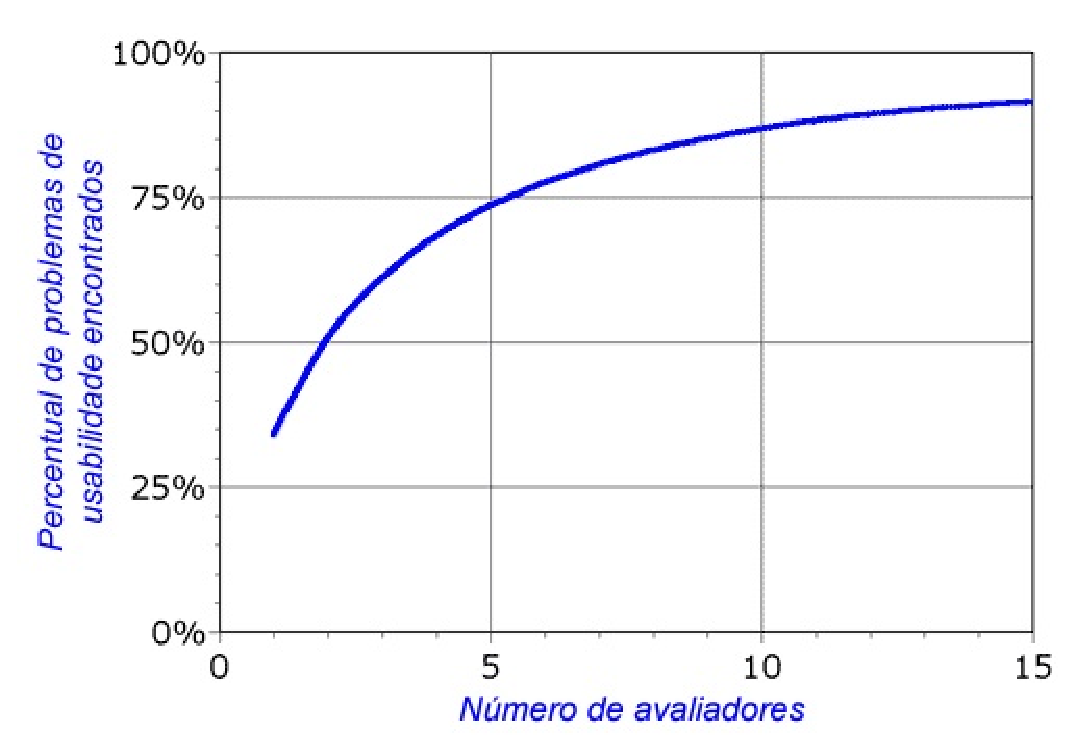
\includegraphics[keepaspectratio=true,scale=0.60]
      {figuras/avaliadores_heuristica.eps}
    \caption{Número de avaliadores~\cite{nielsen1994}}
    \label{avaliadores}
\end{figure}

	A avaliação heurística requer pouco planejamento e pode fazer parte de um processo interativo de um projeto e aplicado em todas as fases de desenvolvimento da interface, mas é preciso que seja avaliado por especialistas de usabilidade com pleno conhecimento nas heurśiticas.
	

\subsubsection{Listas de Verificação}

	Permitem que profissionais que não necessariamente sejam especialistas em ergonomia identifiquem problemas menores e repetitivos das interfaces. As normas 9241, partes 10 a 17, fornecem listas de verificação de ergonomia bem definidas, assim como as fornecidas pelo site Ergolist ~\cite{cybis2010}.
	
	
%Verificar as paginas 216 - cybis

\subsubsection{Percurso Cognitivo}

Percurso cognitivo é um método de inspeção de usabilidade que tem como objetivo avaliar a interface considerando a facilidade da interface. A finalidade do percurso cognitivo é fazer com que o design de interação seja fácil de aprender por meio da exploração.

Os inspetores aplicam uma lista de verificação orientada à tarefa interativa, abordando os processos cognitivos que se estabelecem quando o usuário a realiza pela primeira vez (KIERAS e POLSON, 1991).
	
%Verificar outras fontes além de Cybis


\subsubsection{Teste de Usabilidade}

	É um dos métodos de teste de experiência do usuário (UX) mais frequentemente utilizado e conhecido entre aqueles que não são projetistas da UX.

	Realizar testes com usuários é o núcleo do Design Centrado no Usuário, pois é através deles que podemos saber se as reais expectativas dos usuários são atendidas ~\cite{santos2012}.

	O Teste consiste em avaliar o desempenho dos usuários na execução de tarefas cuidadosamente preparadas, tarefas estas dentro do escopo do sistema. Esse desempenho pode ser avaliado no quesito, número de erros e tempo de execução da tarefa, questionários e entrevistas também podem ser utilizados. (verificar fonte)

	Existe alguns passos comuns que devem ser seguidos para a execução dos testes de usabilidade:

\begin{itemize}

\item \textbf{Escolher abordagem}

	Existem vários tipos de testes de usabilidade, mas sabe-se que todos eles têm algo em comum, que é observar as pessoas utilizando algo.As abordagens de pesquisa podem ser de dois tipos: quantitativa ou qualitativas. 

	Pesquisas quantitativas são focadas nos dados numéricos e é voltada para fornecer alta confiança e resultados repetidos dentro de seus grupos de usuários.É preciso ter o envolvimento de um número maior de participantes para contar as variações que você encontrará de indivíduo para indíviduo ~\cite{unger2009}.

	Os testes quantitativos são como experimentos cientificos que precisam ser rigorosos ou os resultados não serão confiáveis. Deve-se definir um protocolo de teste e segui-lo consistentemente para todos os participantes ~\cite{krug2010}.

	As pesquisas qualitativas não são focadas em níveis de segurança e da possibilidade de repetição, mas sim ganhar contexto e percepção considerando o comportamento do usuário.Ela depende da interpretação do projetista sobre as descobertas, a intuição e o senso comum ~\cite{unger2009}.

	Nos testes qualitativos você tenta minimizar a quantidade de interação com o participante para evitar a influência nos resultados ~\cite{krug2010}.

	Para os testes de usabilidade é possível utilizar qualquer uma das abordagens, mas a qualitativa é a mais acessível para aqueles que não tiveram um treinamento em métodos científicos mais formais e oferece uma rica fonte de dados ~\cite{unger2009}.

	Foi encontrado na literatura o teste de usabilidade "faça você mesmo" que são testes qualitativos onde o objetivo não é provar algo ma sim ter idéias que permitem que você melhore o que você está usando. O teste "faça você mesmo" é uma combinação excelente com os métodos ágeis. 

	O grande desafio encontrado no teste de usabilidade em um ambiente ágil é que parece que é preciso estar sempre planejando à frente das rápidas mudanças feitas pelos programadores e que não tem tempo para a prototipagem.


\item \textbf{Planejar a pesquisa}

Algumas questões devem ser respondidas ao criar o teste de usabilidade: Estas questões te ajudam a oferecer foco e escopo.Abaixo algumas perguntas que devem ser respondidas no planejamento de sua pesquisa:

\begin{itemize}
\item Defina seu objetivo: Por que você está testando? %Cap2
\item Defina Usuários: Quem você está testando? %Cap6e7
\item Defina o método para representar sua aplicação: O que você está testando?
\item Quais informações você está reunindo? 
\end{itemize}

Nas pesquisas qualitativas geralmente queremos compreender as questões que os usuários podem encontrar, os níveis de frustações que eles podem experimentar e a gravidade de um problema em particular. Para os testes qualitativos devem se pensar em medidas que serão possíveis de ser respondidas com cinco usuários ~\cite{unger2009}. 

	\begin{itemize}
		\item Taxa de Sucesso: O grau em que o usuário foi capaz de completar a tarefa?
		%Pode-se detalhar com mais informações sobre o que seria a taxa de sucesso, e o que é considerado o sucesso.
		\item Satisfação do usuário
	\end{itemize}

\item \textbf{Usuários}

Existem algumas diretrizes que podem ser adotadas para a definição da quantidade de usuários. Jacob Nielsen definiu algumas dessas diretrizes:

\begin{itemize}
\item No teste quantitativo planeje uma quantidade maior de participantes. Em média 20 por rodada de pesquisa.
\item No teste qualitativo é suficiente ter entre 5 e 8 participantes.
\end{itemize}

	Em seu livro Simplificando as coisas que parecem complicadas, Krug defende a ideia de que três usuários são ideais para realização de testes de usabilidade para quem está realizando o teste por conta própria. Ele afirma que é mais fácil encontrar três participantes do que uma quantidade maior e que é bem provável que eles já encontrem muitos dos problemas significaticos relacionados as tarefas que você está testando.

	Em equipes ágeis, o teste com o usuário é realizado com o cliente do projeto e envolve o especialista em usabilidade como mediador do teste ~\cite{santos2012}

\item \textbf{Recutramento e logística}

Depois de ter feito o plano de pesquisa e definido os tipos de usuários que podem ser inseridos na pesquisa é hora de recrutar os participantes.
Para o recrutamento de participantes é interessante gerar uma lista com os potenciais participantes do teste. Essa lista pode vir de usuários registrados do site da empresa relacionada; informações de contatos do cliente; e-mails para conhecidos que tenha relação com o assunto do teste; requisições em pequenas pesquisas que pré-qualificam os participantes, e etc.~\cite{unger2009}.

Você pode realizar uma filtragem com os participantes potenciais antes de seleciona-los. As perguntas do questionário de filtragem devem ser voltadas para:

	\begin{itemize}
	\item Garantir que o participante seja um usuário das funções em que você está testando.
	\item Determinar se ele se encaixa em um dos seus grupos de usuários.
	\item Ajudar a ter uma boa mistura de participantes.
	\end{itemize}

O questionário de perfil de usuário pode ser utilizado para realizar essa filtragem de participantes.


\item \textbf{Criação de guias de discussão}

Para a execução do teste de usabilidade é preciso que as instruções estejem claras aos participantes, contendo todas as informações específicas que ele precisará para completar as tarefas com sucesso.

Os seus materiais de teste deve incluir:

	\begin{itemize}
		\item Formulário de consentimento para gravação de vídeo
		\item Guia de discussão para o participante, com tarefas detalhadas e perguntas sobre a satisfação do usuário.
		\item Questionários
	\end{itemize}

\item \textbf{Facilitação}

\item Análise e apresentação dos resultados;
\item Criação de recomendações.

\end{itemize}


%------------------------------------------------------------%
	 

\section{Considerações Finais}


	




